\subsection{Applying Color Marks}
\label{sec:dataset-material-feature}
This work focuses on analyzing how views of the same objects but with different color marks contribute to the classification.
Hence, their information content and significance is evaluated.
This section covers how those color marks are applied.
First, duplicates of every object are created.
This is a trivial task because it can be done by rendering the native object first and then the colored one.
In CAD modeling, objects or faces, in particular, are assigned a material with a color that reacts to light which produces shadows.
Hence, coloring single faces differently becomes the chosen approach for applying color marks due to its simplicity.
However, a well-suited face for being colored needs to be found.
In the following those faces are referred to as an optimal face.
It is important to filter all faces of an object by their area size.
Otherwise, unremarkable ones are probably chosen.
\figref{fig:face-area-filter} illustrates this scenario and the results of several thresholds.
\begin{figure}
	\centering
	\begin{subfigure}{.32\textwidth}
		\centering
		
\includegraphics[width=\textwidth]{images/face_area_unfiltered.png}
		\caption{Unfiltered}
		\label{fig:face-area-unfiltered}
	\end{subfigure}
	\begin{subfigure}{.32\textwidth}
		\centering
		
\includegraphics[width=\textwidth]{images/face_area_mean.png}
		\caption{Face Area Mean}
		\label{fig:face-area-mean}
	\end{subfigure}
	\begin{subfigure}{.32\textwidth}
		\centering
		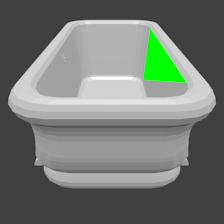
\includegraphics[width=\textwidth]{images/face_area_max_dependent.png}
		\caption{Max Face Area Dependent}
		\label{fig:face-area-max-dependent}
	\end{subfigure}
	\caption[Threshold setup for filtering faces by their area size]{Threshold setup for filtering faces by their area size. The first face that meets the requirement is colored.}
	\label{fig:face-area-filter}
\end{figure}
If faces are not filtered at all, any face can result in being the optimal one.
However, it is not guaranteed that this face has a decent size and can be seen properly.
Like in \figref{fig:face-area-unfiltered} the optimal face is comparatively small to the whole model.
Accepting only faces as the optimal face, that have at least the size of the mean of all faces lead to a result like in \figref{fig:face-area-mean}.
The optimal face can be seen more easily than before, but this threshold often results in long and slender optimal faces.
This is due to the fact, that at least the extracted object classes are mostly modeled with faces in such a shape.
Hence, filtering by the mean of the faces increases the probability to choose such a face as an optimal one.
Therefore, a threshold of above the mean is desired to skip all those long and slender faces like it is shown in \figref{fig:face-area-max-dependent}.
Additionally, larger faces should be preferred.
Thus, the area of the optimal face has to satisfy
\begin{equation}
	\alpha_{\text{opt}} > (\alpha_{\text{mean}} + \alpha_{\text{max}}) \cdot \lambda
\end{equation}
where $\alpha_{\text{mean}}$ and $\alpha_{\text{max}}$ are the mean and maximum of all face areas, respectively, and $\lambda$ a scalar.
With $\lambda = 0.3$ satisfying results are achieved.

Furthermore, it needs to be guaranteed, that the optimal face is visible in at least one view and not visible in at least one view.
This is validated by casting rays from the camera center onto the possible optimal face for every camera position that was defined in \secref{sec:dataset-rendering}.
In brief, if the rays hit the face, the face is visible.
Fortunately, there is a function in Blender performing this approach and returning among others the index of the face that is hit.
However, this cannot be performed for every pixel of a face due to performance issues.
Thus, the trade-off against accuracy is only checking the vertices defining the face.
This can raise errors, though, because a vertex can define multiple faces and it is not certain which face index the function returns.
Hence, checkpoint vertices $\vec{p}_{fi}$ are defined for each face $\mathbb{F}_f = (\vec{v_{f1}}, \vec{v_{f2}}, \vec{v_{f3}})$.
Those are initialized with the coordinates of the vertices $\vec{v}_{fi}$ and slightly moved to the center of the face.
Their actual position is calculated by 
\begin{equation}
	\vec{p}_{fi} = \vec{v}_{fi} + 0.05 \cdot (\vec{v}_{fo} - \vec{v}_{fi})
\end{equation}
where $\vec{v}_{fi}$ is the related vertex and $\vec{v}_{fo}$ the center of the face.
If the ray cast is valid for at least one checkpoint the face is supposed to be visible.
If all rays hit the wrong face, the current face is supposed to be not visible.
As soon as both conditions are satisfied for the examined face among all views, it becomes the optimal face.
Otherwise, the next possible face is investigated.
If the conditions are never satisfied for each possible face, the object is skipped at all.

It is noticed, that some models have duplicated faces.
That are different faces, that are described with the same coordinates as other faces.
Hence, those faces are identical and lie into each other.
If only one of them is colored, rendering issues as visualized in \figref{fig:optimal-face} emerge, because the rendering engine does not know, which color should be rendered on the surface.
Thus, if an optimal face has corresponding identical faces, all of them need to be part of the optimal face and colored as well.
In \figref{fig:optimal-face-single} only one of two identical faces is colored, which leads to the noticeable transparency effect.
That is one of the brighter effects, though.
It is also possible that one optimal face is shown normally and only on the edge rendering issues are visible like a dotted line with the colors of the related identical faces. 
Nevertheless, any of these effects could induce false correlations into the dataset that are not available on real-world objects, hence, leading to a not practical network.
Thus, in \figref{fig:optimal-face-all} the colors of all identical faces are changed, which leads to realistic color representations.
\begin{figure}
	\centering
	\begin{subfigure}{.49\textwidth}
		\centering
		
\includegraphics[width=.7\textwidth]{images/optimal_face_single.png}
		\caption{Single Optimal Face}
		\label{fig:optimal-face-single}
	\end{subfigure}
	\begin{subfigure}{.49\textwidth}
		\centering
		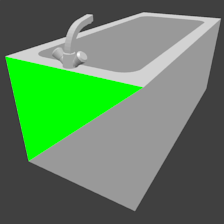
\includegraphics[width=.7\textwidth]{images/optimal_face_all.png}
		\caption{All Optimal Faces}
		\label{fig:optimal-face-all}
	\end{subfigure}
	\caption{Color manipulation on duplicated optimal faces}
	\label{fig:optimal-face}
\end{figure}

Moreover, two color marks are applied on an object for examining how this changes the impact of views on the classification.
Hence, for applying a second color mark on a model, another optimal face or faces, respectively, needs to be found.
A requirement for this is the presence of only one color feature in a single view.
Due to the automation of the rendering, a reliable solution is necessary.
One approach would be using the other side of the surface of the first optimal face.
However, this fails if the surface has a thickness of more than a single face.
Then the next face along its normal needs to be found by ray casting and then the visibility of this face needs to be verified.
Thus, this process leads to excessive ray cast validations and therefore is not pursued.
However, it is considered, that faces at a similar location as the original optimal face are well-suited as well.
Thus, the choices of further optimal faces are narrowed down by sorting all remaining faces by their distance from their center to the center of the first optimal face in descending order.
The intention is that choosing faces with the largest distances result in either an opposite face or in a face that is that far away to not be visible at the same time as the first optimal face.
Of course, the tasks of checking the visibility and finding identical faces are performed on the new face as well.
If no additional optimal face is found, the model is skipped, although, this never happened during execution.